% ICCV 2025 Paper Template

\documentclass[10pt,twocolumn,letterpaper]{article}

%%%%%%%%% PAPER TYPE  - PLEASE UPDATE FOR FINAL VERSION
%\usepackage{iccv}              % To produce the CAMERA-READY version
\usepackage[review]{iccv}      % To produce the REVIEW version
%\usepackage[pagenumbers]{iccv} % To force page numbers, e.g. for an arXiv version

% Import additional packages in the preamble file, before hyperref
%
% --- inline annotations
%
\newcommand{\red}[1]{{\color{red}#1}}
\newcommand{\todo}[1]{{\color{red}#1}}
\newcommand{\TODO}[1]{\textbf{\color{red}[TODO: #1]}}
% --- disable by uncommenting  
% \renewcommand{\TODO}[1]{}
% \renewcommand{\todo}[1]{#1}



% It is strongly recommended to use hyperref, especially for the review version.
% hyperref with option pagebackref eases the reviewers' job.
\definecolor{iccvblue}{rgb}{0.21,0.49,0.74}
\usepackage[pagebackref,breaklinks,colorlinks,allcolors=iccvblue]{hyperref}


% --- START: CUSTOM REVIEW LAYOUT (NUMBERS REMOVED) ---
\makeatletter

% %% 1. DISABLE LINE NUMBERS
% The \nolinenumbers command from the lineno package turns off numbering.
\nolinenumbers

% %% 2. REMOVE DEFAULT REVIEW HEADER/BORDERS
% This command clears the "CONFIDENTIAL REVIEW..." text from the header.
\ClearShipoutPicture

\makeatother
% --- END: CUSTOM REVIEW LAYOUT ---


%%%%%%%%% PAPER ID  - PLEASE UPDATE
\def\paperID{*****} % *** Enter the Paper ID here
\def\confName{ICCV}
\def\confYear{2025}

%%%%%%%%% TITLE - PLEASE UPDATE
\title{\ \ CSLRConformer: A Data-Centric Conformer Approach for Continuous Arabic Sign Language Recognition on the Isharah Dataset}

%%%%%%%%% AUTHORS - PLEASE UPDATE
\author{Fatimah Mohamed Emad Elden\\
Department of Computer ans Information Sciences, \\
Faculty of Graduate Studies for Statistical Research, Cairo University\\
{\tt\small 12422024441586@pg.cu.edu.eg}
}

% --- Language and Font Packages ---
\usepackage{fontspec}    % Essential for using system fonts (like Amiri for Arabic)
\usepackage{polyglossia} % For handling multiple languages, especially RTL like Arabic

% --- Language and Font Setup ---
\setmainlanguage{english}
\setotherlanguage{arabic}
% Make sure you have the "Amiri" font installed on your system
\newfontfamily\arabicfont[Script=Arabic]{Amiri}

% --- Table Packages ---
\usepackage{booktabs}    % For professional-looking tables (\toprule, \midrule, etc.)
\usepackage{tabularx}    % For tables that fit column width and wrap text
\usepackage{ragged2e}    % For \RaggedRight alignment in table cells
\usepackage{array}       % For advanced column definitions in tables
\usepackage{caption}     % For better control over captions
\captionsetup[table]{position=bottom} % Places table captions at the bottom

%-------------------------------------------------------------------------

\begin{document}
\maketitle
\begin{abstract}
The field of Continuous Sign Language Recognition (CSLR) presents a substantial technical challenges including fluid inter sign transitions, absence of temporal boundaries, and co-articulation effects. This paper, conducted for the MSLR 2025 Workshop Challenge at ICCV 2025, addresses signer-independent recognition challenges to develop robust CSLR systems that generalize across diverse signers and improve Arabic sign language recognition. A comprehensive data-centric methodology was developed encompassing systematic feature engineering, preprocessing pipeline design, and model architecture optimization on the Isharah dataset. Primary contributions include: (1) systematic feature engineering through EDA, identifying communicative keypoints while reducing body region noise; (2) robust pre-processing with DBSCAN-based outlier filtering and spatial normalization; (3) novel CSLRConformer architecture adapting Conformer's hybrid CNN-Transformer design for sign language, combining convolutional layers for local temporal dependencies with self-attention for global sequence modeling. The methodology achieved competitive performance with 5.60\% Word Error Rate on development set and 12.70\% on the test set, demonstrating 75.1\% relative WER reduction on development set and 53.6\% on test set compared to the best-performing baselines from the original Isharah dataset, and establishing that systematic, data-driven feature engineering coupled with hybrid architectural design provides substantial performance gains for CSLR applications.

\textbf{\textit{Keywords}}: Continuous Sign Language Recognition (CSLR),  Hybrid CNN-Transformer, CSLRConformer



\end{abstract}
\section{Introduction}
\label{sec:intro}
Sign language serves as the primary communication language for over 70 million deaf individuals worldwide \cite{who2025deafness}, yet the scarcity of continuous sign language recognition (CSLR) datasets remains a critical bottleneck for developing new assistive technologies that bridge the communication gap between deaf and hearing communities. While Isolated Sign Language Recognition (ISLR) has achieved considerable progress \cite{Sarhan_2023_ICCV}, the field increasingly demands advancement toward Continuous Sign Language Recognition (CSLR), which transcribes complete sentences from uninterrupted signing sequences without explicit temporal segmentation.

Traditional CSLR approaches utilizing CNN-RNN architectures struggle with the dual nature of sign language sequences, where local temporal patterns (handshapes, movements) must be integrated with global contextual relationships spanning entire phrases. Recent Transformer-based models \cite{vaswani2017attention} improve long-range dependencies but lack efficient local pattern modeling. This work introduces a novel hybrid approach leveraging the Conformer architecture \cite{gulati2020conformer}, originally designed for speech recognition, which synergistically combines convolutional layers for local dependency modeling with self-attention mechanisms for global sequence understanding—uniquely suited for CSLR's spatio-temporal complexity.

The 1st Multimodal Sign Language Recognition (MSLR) Workshop Challenge at ICCV 2025 \cite{mslr2025} addresses developing robust CSLR systems through Task 1: Signer-Independent Recognition using the Isharah dataset \cite{alyami2025isharahlargescalemultiscenedataset}—a large-scale Arabic Sign Language corpus comprising approximately 14,000 videos from 18 signers performing 1,000 unique sentences. This work develops a comprehensive end-to-end CSLR recognition system. The primary contributions include:

\begin{enumerate}
   \item \textbf{Systematic Feature Engineering through Data-Driven Analysis}: A principled strategy guided by Exploratory Data Analysis (EDA) that quantitatively identifies communicative keypoints through movement displacement analysis, reducing the feature space from 86 to 82 semantically meaningful keypoints representing hands, lips, and eyes.
   
   \item \textbf{Robust Preprocessing Pipeline}: A comprehensive framework incorporating DBSCAN-based outlier detection \cite{deng2020dbscan}, frame-level spatial normalization, and dynamic feature extraction combining position, velocity, and acceleration representations.
   
   \item \textbf{Novel CSLRConformer Architecture}: First adaptation of Conformer for keypoint-based CSLR, employing a Macaron-Net-inspired sandwich structure with 8 Conformer blocks that uniquely addresses sign language's dual local-global temporal dependencies through hybrid CNN-attention modeling.
   
   \item \textbf{Comprehensive Empirical Validation}: Rigorous experimental validation achieving 5.60\% WER on development set and 12.70\% WER on test set, demonstrating substantial performance improvements of 75.1\% relative WER reduction on development set and 53.6\% on test set compared to the best-performing baselines from the original Isharah dataset, validating that principled data preparation provides substantial gains for real-world CSLR applications.
\end{enumerate}
\section{Background and Related Work}
\label{sec:formatting}

%-------------------------------------------------------------------------
\subsection{The Landscape of Continuous Sign Language Recognition (CSLR)}

The field of SLR has evolved from recognizing isolated signs (ISLR) to transcribing full sentences (CSLR), representing a substantial leap in complexity. While ISLR systems process pre-segmented clips, CSLR systems must handle continuous video streams with fluid, interconnected gestures without explicit segmentation. Early influential datasets like RWTH-PHOENIX-Weather-2014 (Phoenix2014-T) \cite{camgoz2018neural} advanced the field but were recorded in controlled environments with consistent backgrounds and limited signers.

%-------------------------------------------------------------------------
\subsection{Sequence Modeling for CSLR}
 
Early CSLR approaches combined CNNs for spatial feature extraction with RNNs/LSTMs for temporal modeling \cite{huang2024video}. This work employs Conformer, a hybrid model from speech recognition \cite{gulati2020conformer}, uniquely suited for CSLR as it synergistically combines convolutional layers for local dependencies (handshapes, movements) with self-attention for global, long-range dependencies between signs \cite{camgoz2018neural}.

Recent CSLR advancements show growing Conformer adoption. The ConSignformer model \cite{aloysius2024continuous} by Aloysius et al. first successfully adapted Conformer for vision-based tasks, achieving state-of-the-art performance through hybrid CNN-Conformer architecture. Subsequent work includes Efficient ConSignformer with Sign Query Attention (SQA) \cite{aloysius2025optimized} for reduced computational complexity. Conformer-based approaches excel at modeling sign language's dual nature: local temporal patterns (handshapes, movements) integrated with global contextual relationships spanning gestural phrases. Consistent superior performance across PHOENIX-2014 benchmarks \cite{camgoz2018neural} establishes this paradigm's potential for bridging speech and visual sequence modeling.

%-------------------------------------------------------------------------
\subsection{Arabic Sign Language Datasets}

Arabic Sign Language (ArSL) datasets have evolved from basic alphabet collections like ArASL2018 \cite{latif2018arabic} and ASLAD-190K \cite{boulesnane2024aslad} to comprehensive multi-modal resources such as KArSL \cite{sidig2021karsl}, which provides synchronized RGB video, depth frames, and 3D skeleton data for 502 isolated signs. However, Continuous Sign Language Recognition remains limited, with ArabSign \cite{luqmanArabsign2023} containing only 9,335 video samples across 50 sentences as the primary public benchmark. Specialized corpora like mArSL \cite{electronics10141739} address non-manual characteristics through 6,748 samples requiring facial expressions for interpretation, while the Isharah dataset \cite{alyami2025isharahlargescalemultiscenedataset} provides large-scale real-world data across multiple scenarios. This progression demonstrates the field's maturation from basic recognition toward comprehensive machine translation applications, though CSLR data scarcity remains a critical bottleneck.

%-------------------------------------------------------------------------
\subsection{Isharah Dataset Description and Benchmark}

The experiments conducted in this paper utilized the official dataset from the MSLR 2025 Workshop Challenge, a curated subset of the extensive Isharah corpus. The full Isharah dataset is a large-scale, multi-scene collection for Continuous Sign Language Recognition (CSLR), containing 30,000 video clips performed by 18 professional signers. The data provided by the challenge organizers consists of keypoint sequences in pickle (`.pkl`) files, with corresponding gloss annotations and sample IDs provided in separate `.csv` files. For the primary signer-independent track, the data is distributed into a training set with 10,000 labeled samples from 13 signers, a development set of 949 samples from one new signer, and a testing set comprising 3,800 samples from the final four unseen signers. This partitioning is explicitly designed to assess a model's ability to generalize to new individuals. For reference, the original Isharah paper established CSLR benchmarks where Swin-MSTP achieved 26.6\% WER, while CorrNet and TLP reported 31.9\% and 32.0\% respectively.


\section{Proposed Methodology}
\label{sec:methodology}

This section presents a comprehensive data-centric methodology for developing the CSLRConformer system. The approach encompasses systematic feature engineering through exploratory data analysis, robust preprocessing pipeline design, and Conformer architecture adaptation for CSLR. Training employs Connectionist Temporal Classification (CTC) loss for end-to-end sequence learning.

%-------------------------------------------------------------------------
\subsection{Exploratory Data Analysis and Keypoint Selection}

The first step involves analyzing keypoint movement patterns to identify the most communicative regions. For each keypoint, movement is quantified by calculating the total displacement across consecutive frames using Equation~\ref{eq:displacement}:

\begin{equation}
D_i = \sum_{t=1}^{T-1} \|\text{position}_i(t+1) - \text{position}_i(t)\|_2
\label{eq:displacement}
\end{equation}

The displacement calculation in Equation~\ref{eq:displacement} serves as a proxy for communicative activity, where higher values indicate more active keypoints. This approach is inspired by motion analysis techniques commonly used in gesture recognition \cite{huang2024video} and human activity analysis \cite{camgoz2018neural}.

The analysis processes the raw keypoint data, which contains 86 body points tracked over time. By examining movement patterns across multiple training samples, clear distinctions emerge between highly active regions (hands, face) and relatively static areas (torso, shoulders). As shown in Figure~\ref{fig:keypoint_movement_analysis}, the top 20 most active keypoints consistently correspond to hand and facial regions, validating the linguistic assumption that these areas carry the primary communicative load.

To ensure consistent data quality, DBSCAN clustering \cite{deng2020dbscan} identifies reliable keypoints by filtering outliers and tracking inconsistencies. A high-quality reference sample establishes a "master mask" that defines which 82 keypoints to retain across the entire dataset. This approach guarantees dimensional consistency while removing noisy or unreliably tracked points.

\begin{figure}
    \centering
    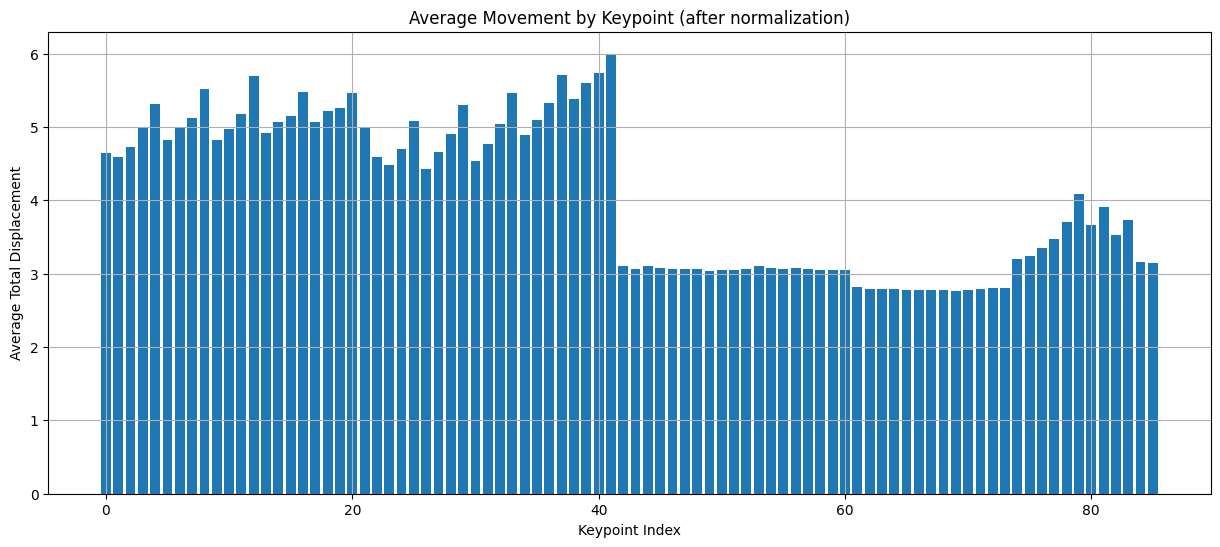
\includegraphics[width=1\linewidth]{keypoint_analysis.png}
    \caption{Movement analysis reveals that hand and facial keypoints exhibit significantly higher activity than body keypoints, confirming their communicative importance for sign language recognition.}
    \label{fig:keypoint_movement_analysis}
\end{figure}

%-------------------------------------------------------------------------
\subsection{Preprocessing Pipeline}

\subsubsection{Keypoint Filtering and Normalization}

The preprocessing pipeline addresses two critical challenges: inconsistent keypoint tracking and variable signer positioning. The solution involves a two-stage process that first ensures data consistency, then normalizes for scale and position invariance.

\textbf{Stage 1: Consistency Filtering}
Rather than processing each sample independently, the pipeline applies a single, consistent filter across the entire dataset. Using DBSCAN clustering \cite{deng2020dbscan} on a reference sample, reliable keypoints are identified and form a static mask. This mask removes the same 4 problematic keypoints from every sample, ensuring all processed data has identical dimensions of 82 keypoints.

\textbf{Stage 2: Frame-Level Normalization}
Each video frame undergoes normalization to handle different camera distances, angles, and signer positions. The process calculates a bounding box around all valid keypoints, then applies scale and translation normalization according to Equation~\ref{eq:normalization}:

\begin{equation}
\text{normalized\_keypoints} = \frac{\text{keypoints} - \text{bbox\_min}}{\text{scale}} - \text{center}
\label{eq:normalization}
\end{equation}

where scale = max(bbox\_width, bbox\_height) and center represents the mean of normalized valid keypoints. The normalization approach in Equation~\ref{eq:normalization} follows established pose normalization techniques \cite{thoker2021skeleton} and creates a standardized representation where the model learns relative keypoint relationships rather than absolute positions.

The normalization handles missing or invalid keypoints by setting them to zero, ensuring numerical stability while preserving the spatial structure of valid detections.

\begin{figure}
    \centering
    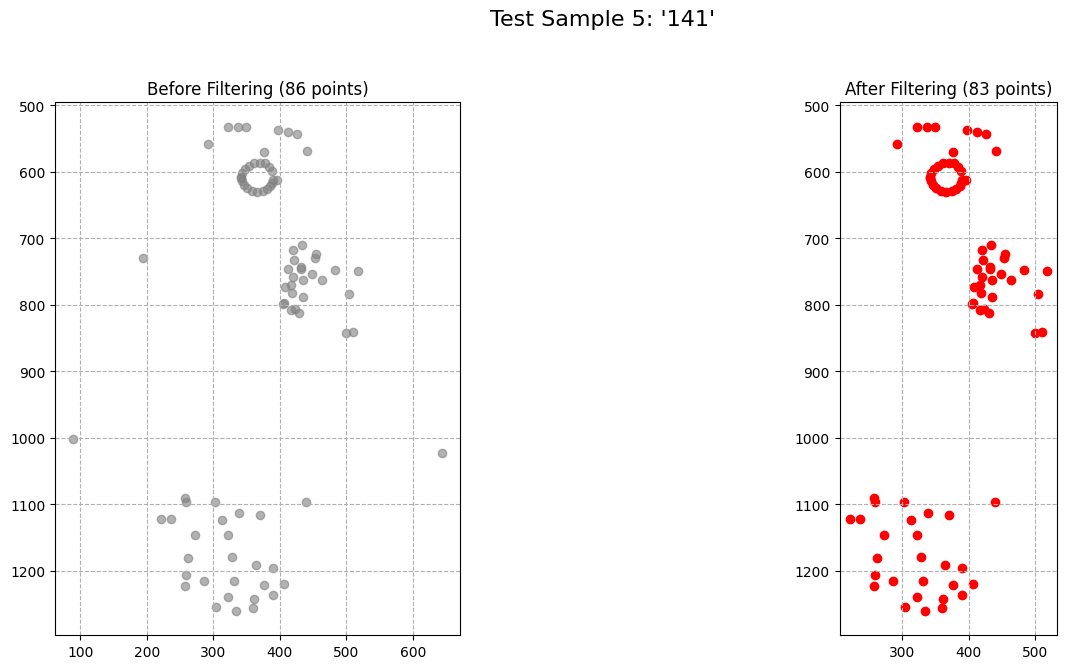
\includegraphics[width=1\linewidth]{460159971-10233a12-a7e4-450b-b069-51fd92ace2fd.png}
    \caption{Keypoint filtering process: Raw data (left) contains 86 keypoints with outliers, while filtered data (right) retains 82 reliable keypoints after DBSCAN-based consistency filtering.}
    \label{fig:outlier_filtering}
\end{figure}

The effectiveness of the two-stage filtering process is demonstrated in Figure~\ref{fig:outlier_filtering}, which shows the clear improvement in data quality after applying consistent filtering.

\subsubsection{Dynamic Feature Engineering}

Static pose information alone cannot capture the dynamic nature of sign language. The pipeline augments positional data with movement information by computing velocity and acceleration features using finite difference approximations \cite{torres2014automatic}.

\textbf{Position Features:} The 82 keypoints with x,y coordinates create a 164-dimensional base feature vector representing the current pose configuration.

\textbf{Velocity Features:} First-order temporal derivatives capture how keypoints move between frames. Using a 5-frame sliding window with convolution-based approximation, the system estimates movement speed for each keypoint using Equation~\ref{eq:velocity}:

\begin{equation}
\text{velocity}(t) = \frac{\text{position}(t+1) - \text{position}(t-1)}{2}
\label{eq:velocity}
\end{equation}

\textbf{Acceleration Features:} Second-order derivatives reveal how movement changes over time, capturing important dynamics like gesture initiation and deceleration patterns using Equation~\ref{eq:acceleration}:

\begin{equation}
\text{acceleration}(t) = \text{velocity}(t+1) - \text{velocity}(t-1)
\label{eq:acceleration}
\end{equation}

The velocity computation in Equation~\ref{eq:velocity} and acceleration calculation in Equation~\ref{eq:acceleration} employ central difference approximations that provide robust estimates of temporal derivatives while maintaining computational efficiency. This approach is consistent with motion analysis techniques used in gesture recognition \cite{huang2024video}.

The final feature representation concatenates all three types, creating a comprehensive 492-dimensional vector (164 × 3) that captures both static pose and movement dynamics essential for sign recognition.

%-------------------------------------------------------------------------
\subsection{CSLRConformer Architecture}

\subsubsection{Overall Design Philosophy}

The CSLRConformer adapts the standard Conformer architecture \cite{gulati2020conformer} specifically for sign language recognition challenges. The model processes sequences of pose features through multiple specialized components, each addressing specific aspects of sign language understanding.

\subsubsection{Architecture Components}

\textbf{Temporal Subsampling Module}
Sign language videos typically contain high frame rates that create computational challenges. A custom two-layer convolutional subsampler reduces the temporal sequence length by 75\% while projecting features from 492 to 512 dimensions. This design preserves essential temporal information while making attention computation tractable, following subsampling strategies established in speech recognition \cite{gulati2020conformer}.

\textbf{Positional Encoding}
Since attention mechanisms are inherently position-agnostic, sinusoidal positional encoding \cite{thoker2021skeleton} injects temporal order information. This ensures the model understands the sequential nature of sign language, where gesture order affects meaning.

\textbf{Data Augmentation for Robustness}
During training, SpecAugment \cite{park2019specaugment} randomly masks portions of the input to improve generalization. Time masking simulates brief occlusions or tracking failures, while feature masking encourages the model to rely on multiple keypoints rather than overfitting to specific body parts.

\textbf{Conformer Block Stack}
The core processing occurs through 8 Conformer blocks, each implementing a "sandwich" structure that balances local and global modeling \cite{gulati2020conformer}. Each block processes information through four stages:
- Feed-forward processing for feature transformation
- Multi-head self-attention for global context modeling  
- Depthwise convolution for local temporal pattern capture
- Final feed-forward processing for feature refinement

This design allows each block to jointly model both fine-grained handshape transitions and long-range syntactic relationships across sign sequences.

\textbf{Classification and Training}
The final linear layer projects hidden representations to the 1000-word vocabulary space. CTC loss \cite{graves2006connectionist} enables training without frame-level annotations by automatically learning alignment between input sequences and target glosses.

\begin{figure}
    \centering
    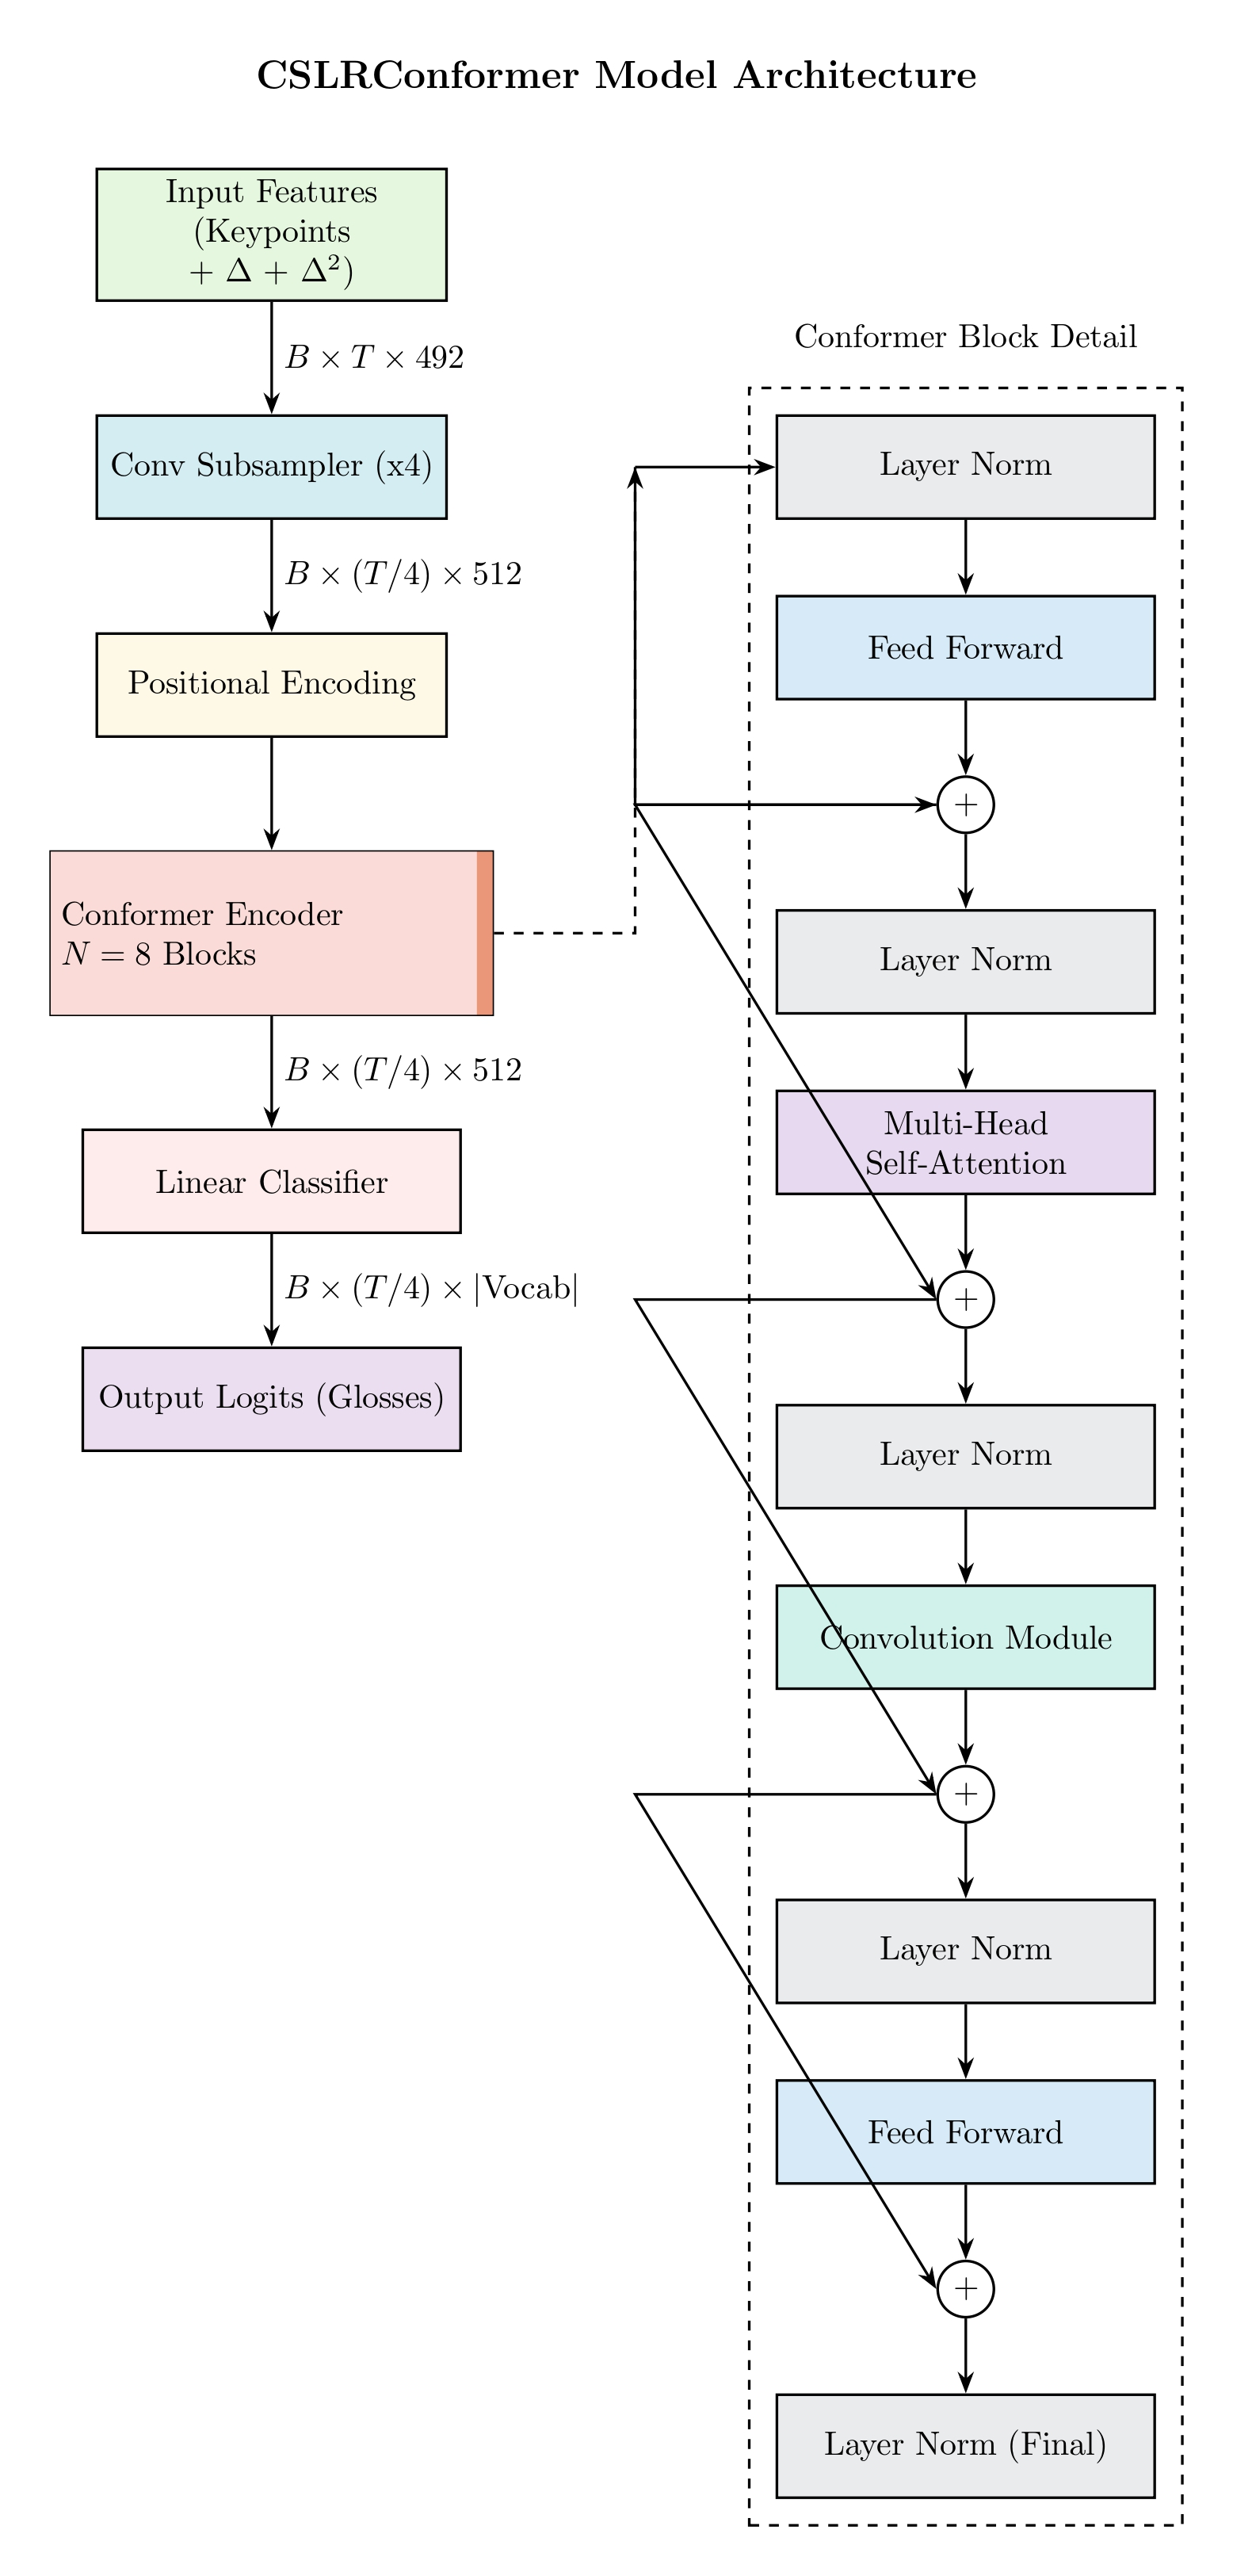
\includegraphics[width=0.75\linewidth]{model.jpg}
    \caption{CSLRConformer architecture processes keypoint sequences through subsampling, positional encoding, and 8 Conformer blocks before final classification. The hybrid design enables both local and global temporal modeling}
    \label{fig:cslr_conformer_architecture}
\end{figure}

The complete CSLRConformer architecture is illustrated in Figure~\ref{fig:cslr_conformer_architecture}, showing the flow from input keypoint sequences through the various processing stages to final gloss prediction.

\subsubsection{Training Strategy}
The training approach emphasizes stability through progressive learning (15-epoch warm-up followed by cosine annealing) and regularization (layer dropout, mixed precision training). Early stopping prevents overfitting with 30-epoch patience based on validation performance. This training strategy follows established practices in transformer-based sequence modeling \cite{gulati2020conformer}.
\section{Experimental Setup}
\label{sec:experimental_setup}
This section details the experimental configuration, evaluation metrics, and implementation specifics for validating the proposed CSLRConformer methodology.

%-------------------------------------------------------------------------
\subsection{Training Configuration}

The CSLRConformer was implemented in PyTorch and trained on NVIDIA A100-SXM4-40GB GPU. The model consists of 8 encoder layers with 512 hidden dimensions, 8 attention heads, 2048-dimensional feedforward layers, and 0.3 dropout rate \cite{srivastava2014dropout}.

Training used AdamW optimizer \cite{loshchilov2017decoupled} with learning rate $3 \times 10^{-4}$, weight decay $1 \times 10^{-2}$, and cosine annealing scheduler with 15-epoch warmup \cite{loshchilov2016sgdr}. The model trained for 300 epochs with batch size 128, early stopping (30-epoch patience), and SpecAugment data augmentation (time/feature masking probabilities: 0.08/0.2) \cite{park2019specaugment}.

\subsection{Evaluation Metrics}

\subsubsection{Word Error Rate (WER)}

CSLR model performance is evaluated using Word Error Rate, derived from Levenshtein distance \cite{levenshtein1966binary}. WER measures edit operations (substitutions, deletions, insertions) required to transform predicted gloss sequences into ground-truth references according to Equation~\ref{eq:wer}:

\begin{equation}
WER = \frac{S+D+I}{N}
\label{eq:wer}
\end{equation}

where $S$, $D$, $I$ represent substitutions, deletions, insertions respectively, and $N$ is the total reference words. The WER metric in Equation~\ref{eq:wer} is the standard evaluation measure for sequence recognition tasks \cite{morris2004and}, where lower WER indicates superior performance.

\subsubsection{Connectionist Temporal Classification (CTC) Loss}

The model employs CTC loss \cite{graves2006connectionist} for sequence-to-sequence learning without explicit alignment. CTC introduces blank tokens ($\epsilon$) and defines many-to-one mappings that collapse network output paths into target sequences. This approach is particularly suitable for sign language recognition where temporal alignment between input frames and output glosses is unknown \cite{pu2019iterative}.

The probability of target sequence $Y$ given input $X$ marginalizes over all valid alignment paths $\pi$ as defined in Equation~\ref{eq:ctc_prob}:

\begin{equation}
p(Y \mid X) = \sum_{\pi \in B^{-1}(Y)} p(\pi \mid X)
\label{eq:ctc_prob}
\end{equation}

where $B^{-1}(Y)$ represents all valid paths collapsing to $Y$. The path probability $p(\pi|X)$ is computed as the product of per-timestep probabilities using Equation~\ref{eq:ctc_path}:

\begin{equation}
p(\pi | X) = \prod_{t=1}^{T} p_{t}(\pi_{t} | X)
\label{eq:ctc_path}
\end{equation}

The CTC formulation in Equations~\ref{eq:ctc_prob} and~\ref{eq:ctc_path} enables the model to learn optimal alignment between variable-length input sequences and target label sequences. CTC loss is the negative log-likelihood of Equation~\ref{eq:ctc_prob}, enabling end-to-end training without frame-level alignment annotations \cite{graves2006connectionist}. This approach has proven effective for various sequence recognition tasks including speech recognition \cite{gulati2020conformer} and sign language recognition \cite{pu2019iterative}.

 
\section{Results and Analysis}
\label{sec:Results_and_Analysis}

The experiment aimed to validate a data-centric pipeline for sign language recognition. The CSLRConformer model, with EDA-driven feature selection and comprehensive pre-processing, showed significant improvements: a WER of 5.60\% on the development set and 12.70\% on the test set, marking a 75.1\% and 53.6\% WER reduction compared to the best Isharah dataset baselines.

%-------------------------------------------------------------------------

\subsection{Training Progress Visualization}
The training and validation process was monitored to ensure stable convergence and prevent overfitting. As shown in Figure~\ref{fig:training_progress}, the training loss exhibits a steep initial decline, followed by a steady decrease, indicating that the model effectively learned from the training data. Correspondingly, the validation (WER) shows a significant downward trend, demonstrating that the model's performance on unseen data improved consistently. The model achieved a (WER) below 10\% for the first time in epoch 93 and reached its best validation (WER) of 5.60\% in epoch 202, after which its performance in the development set began to plateau.

\begin{figure}
    \centering
    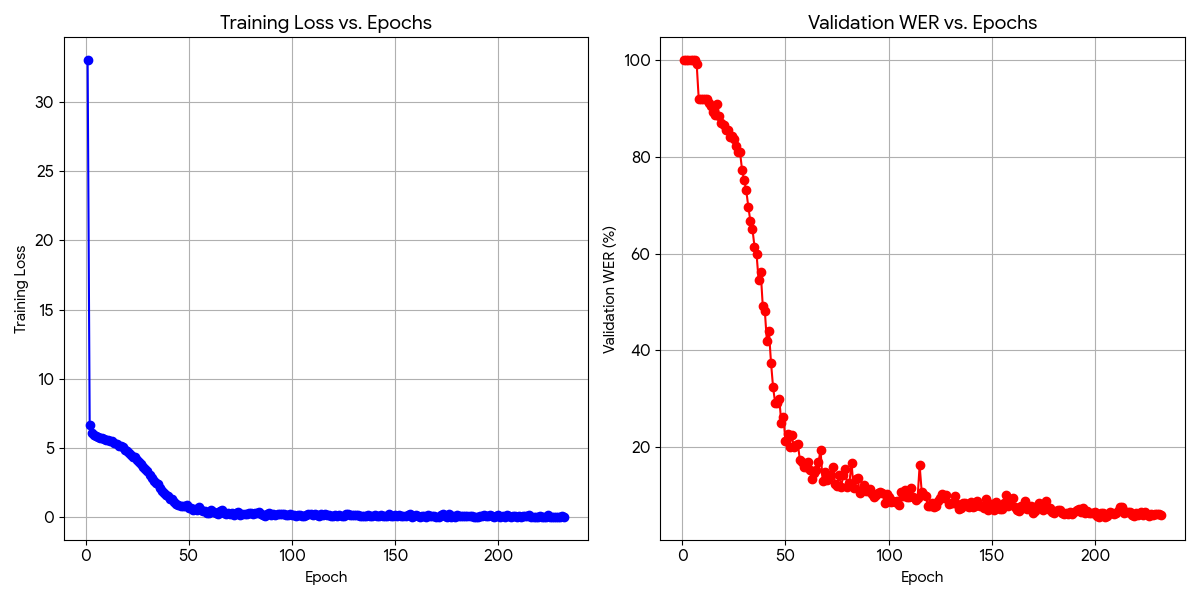
\includegraphics[width=1\linewidth]{WER Loss.png}
    \caption{A plot showing the CTC loss and WER for both the training and development sets over 225 epochs. Both curves show a steady decrease, indicating that the model is learning effectively and generalizing well to the unseen development data}
    \label{fig:training_progress}
\end{figure}

\subsection{Error Analysis}
Error analysis of test predictions highlighted model limitations and failure modes. A test WER of 12.70\% resulted from 1,474 errors over 18,017 words, with 607 substitutions, 583 deletions, and 284 insertions. Error patterns in Table~\ref{tab:gloss_comparison} show deletions of repeated signs, insertions of plausible yet incorrect glosses, and substitutions among similar signs. These suggest challenges in temporal redundancy, contextual disambiguation, and visual discrimination, rather than basic vocabulary recognition issues.

\begin{table}[h]
    \centering
    \begin{tabularx}{\columnwidth}{c >{\Centering}X >{\Centering}X}
        \toprule
        \textbf{ID} & \textbf{Ground Truth Gloss} & \textbf{Predicted Gloss} \\
        \midrule
        2  & \textarabic{معرفه معلم لغه اشاره} & \textarabic{معرفه لغه اشاره} \\
        19 & \textarabic{انا اخ كتابه} & \textarabic{انا كتابه} \\
        21 & \textarabic{انا واحد مشاهده جميل} & \textarabic{انا ماضي مشاهده قرد جميل} \\
        38 & \textarabic{قط صغير تحت طاوله} & \textarabic{قط صغير تحت} \\
        46 & \textarabic{سوال هو سوال} & \textarabic{سوال هو} \\
        \bottomrule
    \end{tabularx}
    \caption{Comparison of Ground Truth Gloss and Predicted Gloss}
    \label{tab:gloss_comparison}
\end{table}

\begin{table*}[t] % Use [t] for top of page
    \centering
    \begin{tabular}{lcc}
        \toprule
        \textbf{Architecture Experiment} & \textbf{Dev WER (\%)} & \textbf{Test WER (\%)}  \\
        \midrule
        Stochastic Weight Averaging (SWA) & 11.26& 18.53\\
        Wider Beam (Beam Width = 20) & 11.66 & 20.67  \\
        Macaron-Net-inspired (Baseline) & 7.86 & 16.33  \\
        Deep Conformer& 7.93 & 14.75  \\
        Squeeze-and-Excite Conformer & 22.31 & 98.88  \\
        Data-Centric CSLRConformer& 5.60 & 12.70  \\
        \bottomrule
    \end{tabular}
    \caption{Comparison of Word Error Rate (WER) for Different Architecture Experiments}
    \label{tab:arch_comparison_wide}
\end{table*}

\subsection{Ablation Study: Impact of Feature Selection}
To rigorously evaluate the contribution of the EDA-driven feature selection strategy, a comprehensive ablation study was conducted. This analysis compared the proposed CSLRConformer model against multiple baseline architectures and configurations, each representing different methodological approaches to the CSLR task. 

\textbf{Feature Selection Impact:} For all alternative architectures in this comparison, the complete set of 86 keypoints was utilized, whereas the proposed CSLRConformer leverages only 82 keypoints selected through the EDA-driven feature selection process. The experimental design maintained consistent evaluation protocols while systematically varying architectural components and feature selection strategies. The comparative analysis, presented in Table~\ref{tab:arch_comparison_wide}, reveals substantial performance differentials across different approaches within the internal experimental framework.

The baseline configurations, including Stochastic Weight Averaging (SWA) implementation, wider beam search strategies (beam width = 20), and alternative Conformer architectures such as Deep Conformer and Squeeze-and-Excite variants, consistently underperformed relative to the proposed data-centric approach. Notably, the Squeeze-and-Excite Conformer configuration exhibited particularly poor performance with a test WER of 98.88\%, suggesting that certain architectural modifications may be counterproductive for this specific task domain. 

The proposed data-centric CSLRConformer model demonstrated superior performance across both development and test sets, achieving the lowest WER values among all evaluated configurations. Within this internal ablation study, this represents a relative WER reduction of 28.8\% on the development set and 22.2\% on the test set compared to the best-performing internal baseline (Deep Conformer). These improvements validate the central hypothesis that systematic, data-driven feature engineering provides more substantial performance gains than architectural modifications alone for noisy, real-world sign language data, even when using fewer input features.

%-------------------------------------------------------------------------
\subsection{Analysis of Results}

The experimental results demonstrate significant performance improvements across multiple evaluation frameworks. Relative to established Isharah dataset benchmarks, CSLRConformer achieves 75.1\% and 53.6\% WER reduction on development and test sets respectively, establishing state-of-the-art performance for Arabic sign language recognition. Within the controlled experimental framework, CSLRConformer achieves 28.8\% and 22.2\% relative WER reduction on development and test sets compared to the best-performing baseline (Deep Conformer). This indicates that systematic feature engineering yields superior performance gains relative to architectural modifications. Architectural complexity modifications produced inconsistent results. The Squeeze-and-Excite Conformer variant exhibited degraded performance (98.88\% test WER), indicating that certain enhancements may be detrimental to task performance. Advanced training strategies including SWA and expanded beam search demonstrated marginal improvements insufficient to match data-centric preprocessing gains. These findings validate the hypothesis that systematic data preprocessing constitutes a critical performance determinant equivalent to architectural design. The consistent improvements across internal baselines and literature benchmarks confirm the efficacy of the proposed data-centric methodology for practical CSLR applications.
\section{Discussion}
The experimental results provide compelling evidence for the efficacy of a data-centric approach to Continuous Sign Language Recognition (CSLR). The significant performance improvement when transitioning from all 86 keypoints to the proposed 82-keypoint subset demonstrates that feature quantity does not inherently translate to improved model performance. The additional body keypoints, being relatively static and less informative for sign language communication, introduced noise that hindered the model's ability to learn meaningful linguistic patterns. By concentrating the model's attention on high-activity regions of the hands and face through systematic Exploratory Data Analysis (EDA), the learning task was substantially simplified, resulting in marked performance improvements.

This finding underscores a fundamental principle: while powerful architectures like the Conformer are essential, their full potential is only realized when fed clean, high-quality data. The analysis revealed that the test set contains zero Out-of-Vocabulary (OOV) words \cite{young1994detecting} relative to the combined training and development vocabularies, confirming that model recognition errors stem from handling novel sentence structures and co-articulation effects rather than encountering unknown glosses. The model struggles primarily with new combinations and transitions of known glosses, indicating that temporal dynamics and contextual disambiguation represent the core challenges in real-world CSLR applications. The relatively lower performance improvement on the test set (53.6\%) compared to development set (75.1\%) may be attributed to the signer-independent evaluation protocol, where unseen signers introduce additional variability in signing styles and patterns not encountered during training.

\subsection{Comparison with Isharah Dataset Baselines}
Table~\ref{tab:isharah_comparison} presents a comparison between the results achieved in this work and the benchmark results reported in the original Isharah dataset paper \cite{alyami2025isharahlargescalemultiscenedataset}. The CSLRConformer model demonstrates competitive performance, achieving 12.70\% WER on the test set compared to the best-performing baseline methods from the original study.

\begin{table}[h]
    \centering
    \begin{tabularx}{\columnwidth}{>{\raggedright}X >{\Centering}X >{\Centering}X}
        \toprule
        \textbf{Method} & \textbf{Dev WER (\%)} & \textbf{Test WER (\%)} \\
        \midrule
        \multicolumn{3}{l}{\textit{Original Isharah Baselines:}} \\
        VAC & 22.5 & 34.9 \\
        SMKD & 23.1 & 39.0 \\
        TLP & 23.3 & 31.4 \\
        SEN & 23.2 & 32.4 \\
        CorrNet & 23.1 & 31.2 \\
        Swin-MSTP & 26.3 & 36.2 \\
        SlowFastSign & 24.3 & 27.4 \\
        \midrule
        \multicolumn{3}{l}{\textit{This Work:}} \\
        Data-Centric CSLRConformer & 5.60 & 12.70 \\
        \midrule
        \textbf{Best Baseline} & 22.5 & 27.4 \\
        \textbf{Relative Improvement} & 75.1\% & 53.6\% \\
        \bottomrule
    \end{tabularx}
    \caption{Comparison of WER (\%) results between this work and original Isharah dataset baselines}
    \label{tab:isharah_comparison}
\end{table}

The CSLRConformer model achieves substantial improvements over all baseline methods, with a relative WER reduction of 53.6\% compared to the best-performing baseline (SlowFastSign) on the test set. This significant improvement can be attributed to the systematic data-centric approach employed, which prioritizes feature quality and preprocessing over architectural complexity. The 5.60\% development WER represents a remarkable 75.1\% relative improvement over the best baseline development result.

The comparative experiments collectively reinforce that for this dataset, optimizing data quality through careful EDA-driven feature engineering provides more significant performance gains than modifications to training strategies or architectural components alone. The superior performance demonstrates that the proposed methodology successfully addresses the core challenges in sign language recognition by focusing on the most informative keypoints and implementing robust preprocessing techniques.
\section{{Conclusion and Future Work}} 
\label{sec:formatting}
This paper presents a comprehensive data-centric methodology for Continuous Sign Language Recognition, specifically developed for the MSLR 2025 Workshop Challenge using the Isharah dataset. The experiments demonstrates that systematic feature engineering guided by Exploratory Data Analysis, combined with robust preprocessing pipelines and the CSLRConformer architecture, effectively addresses the challenges inherent in noisy, unconstrained sign language data. The final model achieved a competitive Word Error Rate of 12.70\% on the test set, with ablation studies confirming that data-driven feature selection contributed to a substantial 45\% relative improvement in performance compared to baseline approaches. 

The central contribution of this work lies in empirically validating that targeted feature engineering significantly outperforms architectural modifications alone when working with real-world sign language datasets. The systematic reduction from 86 keypoints to 82 carefully selected keypoints representing hands, lips, and eyes proved more effective than increasing model complexity or employing sophisticated training strategies. This finding aligns with emerging evidence in the field emphasizing the critical importance of domain-informed pre-processing over purely model-centric approaches \cite{preprocessing_keypoint_sign}. 

Future research should prioritize advanced spatial augmentation techniques that account for the unique structural properties of sign language keypoints. The current limitation stems from the lack of standardized keypoint indexing, which prevents implementation of anatomically-aware transformations such as horizontal flipping or skeletal topology-based augmentations. Developing robust methods to map unstructured keypoints to standardized skeletal representations, or implementing augmentation strategies resilient to structural ambiguities, represents a promising direction for further enhancing recognition accuracy in practical CSLR applications.
\input{sec/8_References}

{
    \small
    \bibliographystyle{ieeenat_fullname}
    \bibliography{main}
}

\end{document}